% Source : http://tex.stackexchange.com/questions/36109/making-tikz-nodes-hyperlinkable

\documentclass{article} 
	\usepackage{tikz}

	\makeatletter
	\newcount\dirtree@lvl
	\newcount\dirtree@plvl
	\newcount\dirtree@clvl
	\def\dirtree@growth{%
		\ifnum\tikznumberofcurrentchild=1\relax
		\global\advance\dirtree@plvl by 1
		\expandafter\xdef\csname dirtree@p@\the\dirtree@plvl\endcsname{\the\dirtree@lvl}
		\fi
		\global\advance\dirtree@lvl by 1\relax
		\dirtree@clvl=\dirtree@lvl
		\advance\dirtree@clvl by -\csname dirtree@p@\the\dirtree@plvl\endcsname
		\pgf@xa=0.5cm\relax % change the length to your needs
		\pgf@ya=-0.75cm\relax % change the length to your needs
		\pgf@ya=\dirtree@clvl\pgf@ya
		\pgftransformshift{\pgfqpoint{\the\pgf@xa}{\the\pgf@ya}}%
		\ifnum\tikznumberofcurrentchild=\tikznumberofchildren
		\global\advance\dirtree@plvl by -1
		\fi
	}
	\tikzset{ %definition of a new style "dirtree"
		dirtree/.style={
			growth function=\dirtree@growth,
			every node/.style={anchor=north},
			every child node/.style={anchor=west},
			edge from parent path={(\tikzparentnode\tikzparentanchor) |- (\tikzchildnode\tikzchildanchor)}
		}
	}
	\makeatother

	\usepackage{hyperref}


\begin{document}

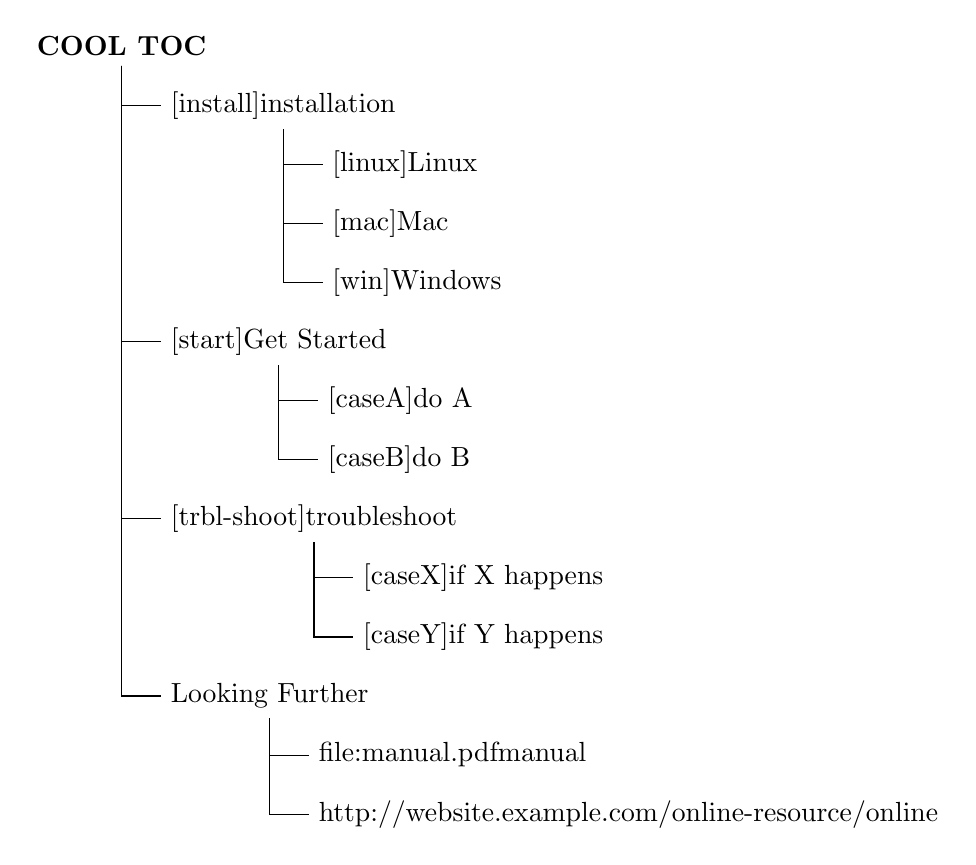
\begin{tikzpicture}[dirtree] % it's what we defined above
	\node {\textbf{COOL TOC}}
		child {
			node {\hyperref[install]{installation} }
				child { node {\hyperref[linux]{Linux}} }
				child { node {\hyperref[mac]{Mac}} }
				child { node {\hyperref[win]{Windows}} }
		}
		child {
			node {\hyperref[start]{Get Started}}
				child { node {\hyperref[caseA]{do A}} }
				child { node {\hyperref[caseB]{do B}} }
		}
		child {
			node {\hyperref[trbl-shoot]{troubleshoot}}
				child {node {\hyperref[caseX]{if X happens}}}
				child {node {\hyperref[caseY]{if Y happens}}}
		}
% I've put the external resources to the end:
		child {
			node {Looking Further}
				child { node {\href{file:manual.pdf}{manual}} }
% This works only, if "manual.pdf" is in the same directory
% as the compiled version of this document.
				child { node {\href{http://website.example.com/online-resource/}{online}} }
		};
\end{tikzpicture}


\section*{Installation}\label{install}

\subsection*{Linux}\label{linux}

Some content.


\subsection*{Mac}\label{mac}

Some content.


\subsection*{Windows}\label{win}

Some content.


\section*{Get started}\label{start}

\subsection*{First: Do A}\label{caseA}

Some content.


\subsection*{Second: Do B}\label{caseB}

Some content.


\section*{Trouble shooting}\label{trbl-shoot}

\subsection*{If X happens:}\label{caseX}

Some content.


\subsection*{If Y happens:}\label{caseY}

Some content.

\end{document}
